\chapter{Perfiles Completamente Desarrollados (Capítulo 5)} \label{apen:desarrollado}

En este apéndice se exponen los perfiles de cantidades de primer y segundo orden (completamente desarrollados), obtenidos vía simulaciones, para los números adimensionales: $\text{Re}_o=2100,3150,4278$; $\text{Pr}=0\text{.}071,0\text{.}71$ y diferentes números de Ri$_b$. 

\subsection*{$\text{Re}=2100$ y $\text{Pr}=0\text{.}71$}

\begin{figure}[H]
  \centering
    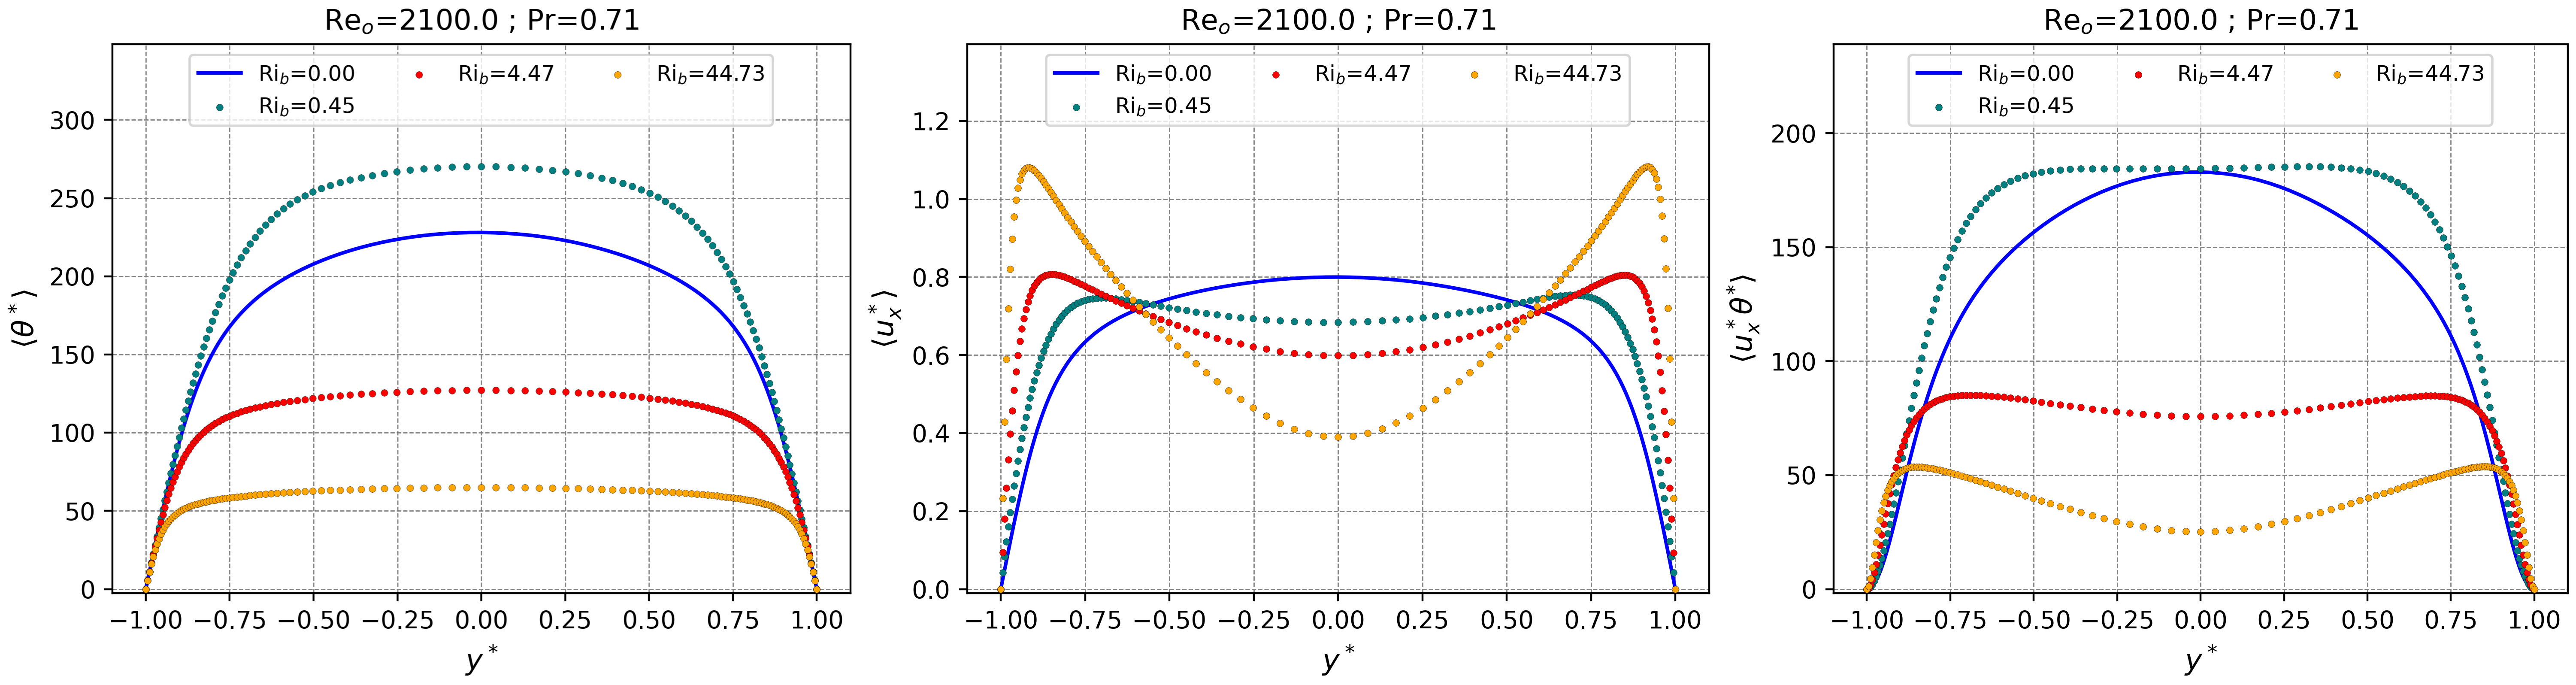
\includegraphics[width=\textwidth]{figures/apendices/developed/Re2100-Pr071_merged_phi-ux-uxphi.png}
  \caption{Perfiles de  $\langle \theta^* \rangle$,  $\langle u^*_x \rangle$ y   $\langle u^*_x \theta^* \rangle$.}
  \label{fig:profs-Re2100-Pr071}
\end{figure}

\begin{figure}[H]
  \centering
    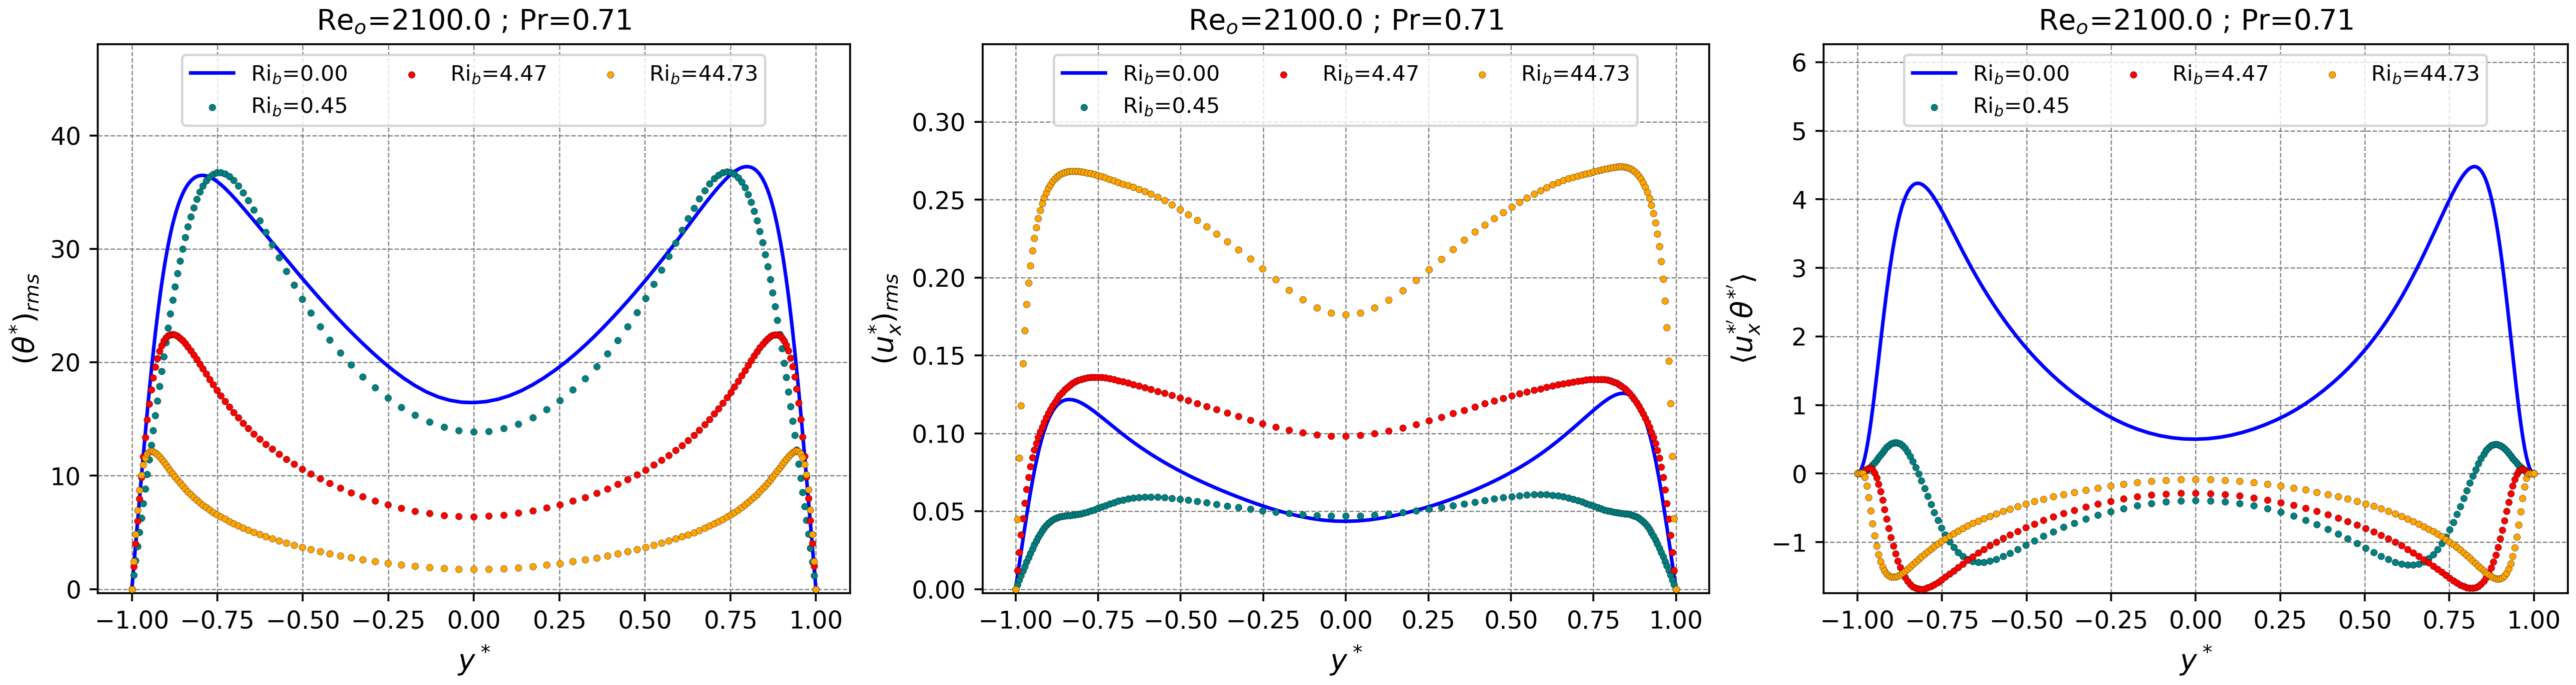
\includegraphics[width=\textwidth]{figures/apendices/developed/Re2100-Pr071_merged_phif-uxf-uxphif.png}
  \caption{Perfiles de  $( \theta^*)_{\text{rms}}$,  $(u^*_x)_{\text{rms}}$ y  $\langle u^{* \prime}_x \theta^{* \prime} \rangle$.}
  \label{fig:profs-Re2100-Pr071}
\end{figure}

\subsection*{$\text{Re}=2100$ y $\text{Pr}=0\text{.}071$}

\begin{figure}[H]
  \centering
    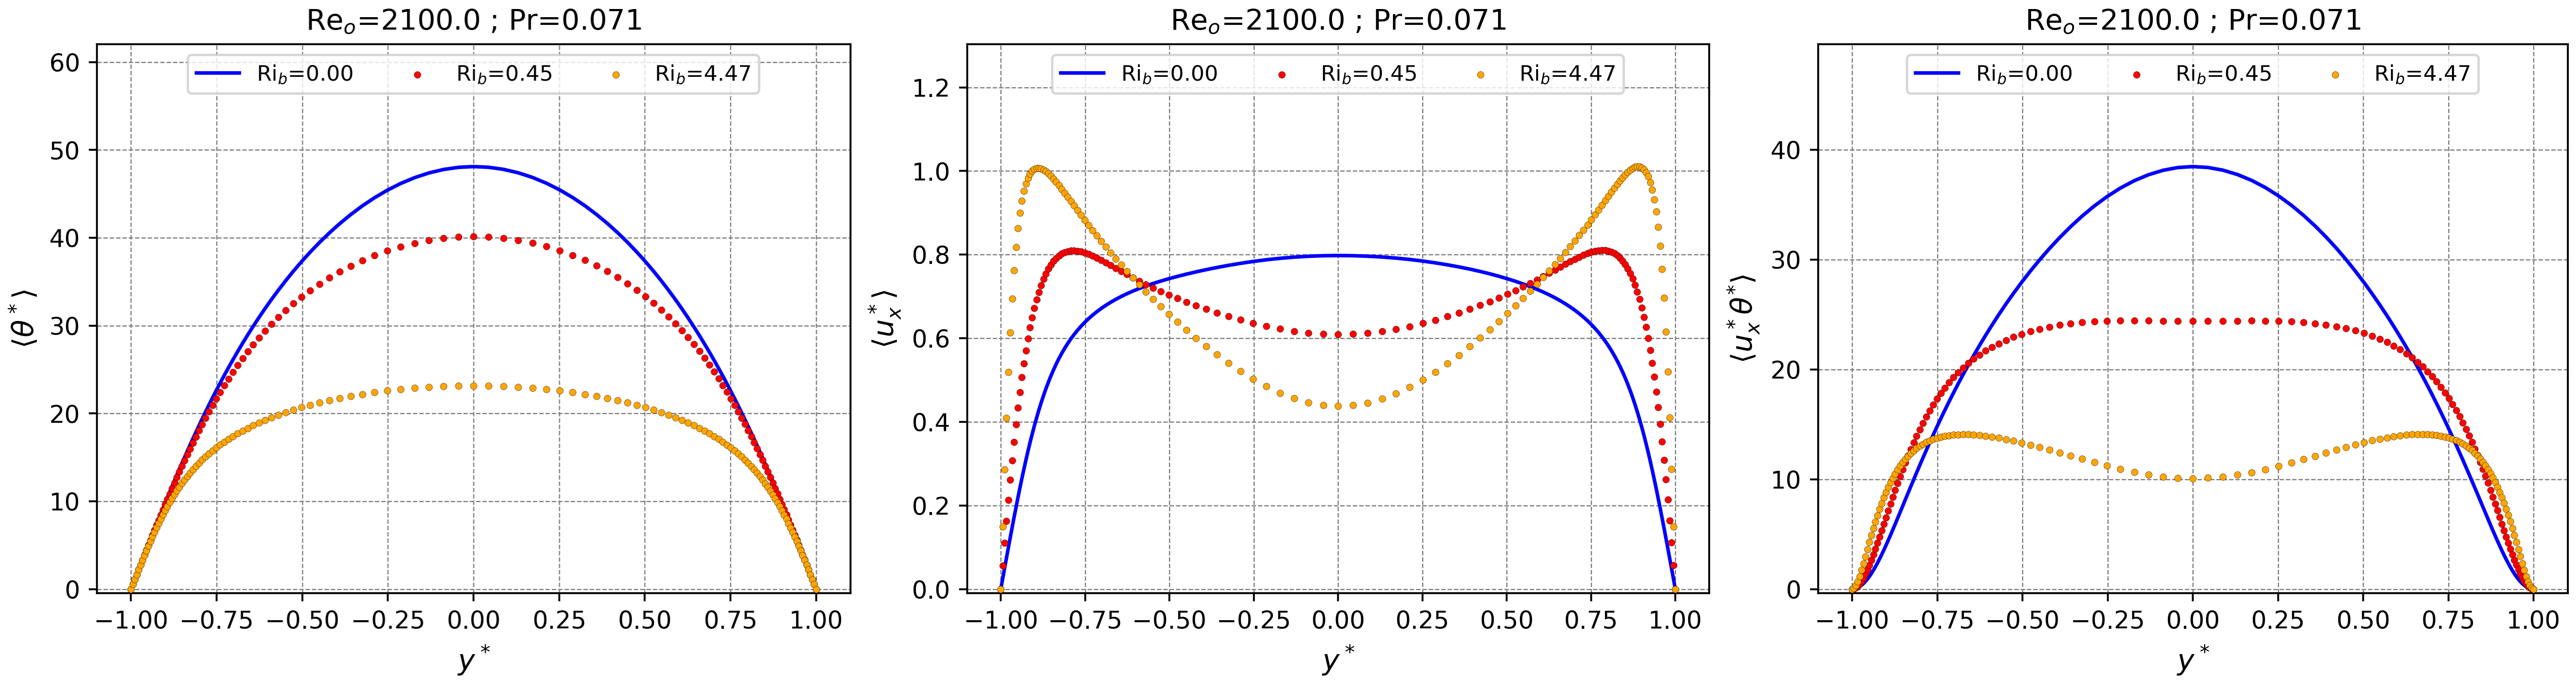
\includegraphics[width=\textwidth]{figures/apendices/developed/Re2100-Pr0071_merged_phi-ux-uxphi.png}
  \caption{Perfiles de  $\langle \theta^* \rangle$,  $\langle u^*_x \rangle$ y   $\langle u^*_x \theta^* \rangle$.}
  \label{fig:profs-Re2100-Pr0071}
\end{figure}

\begin{figure}[H]
  \centering
    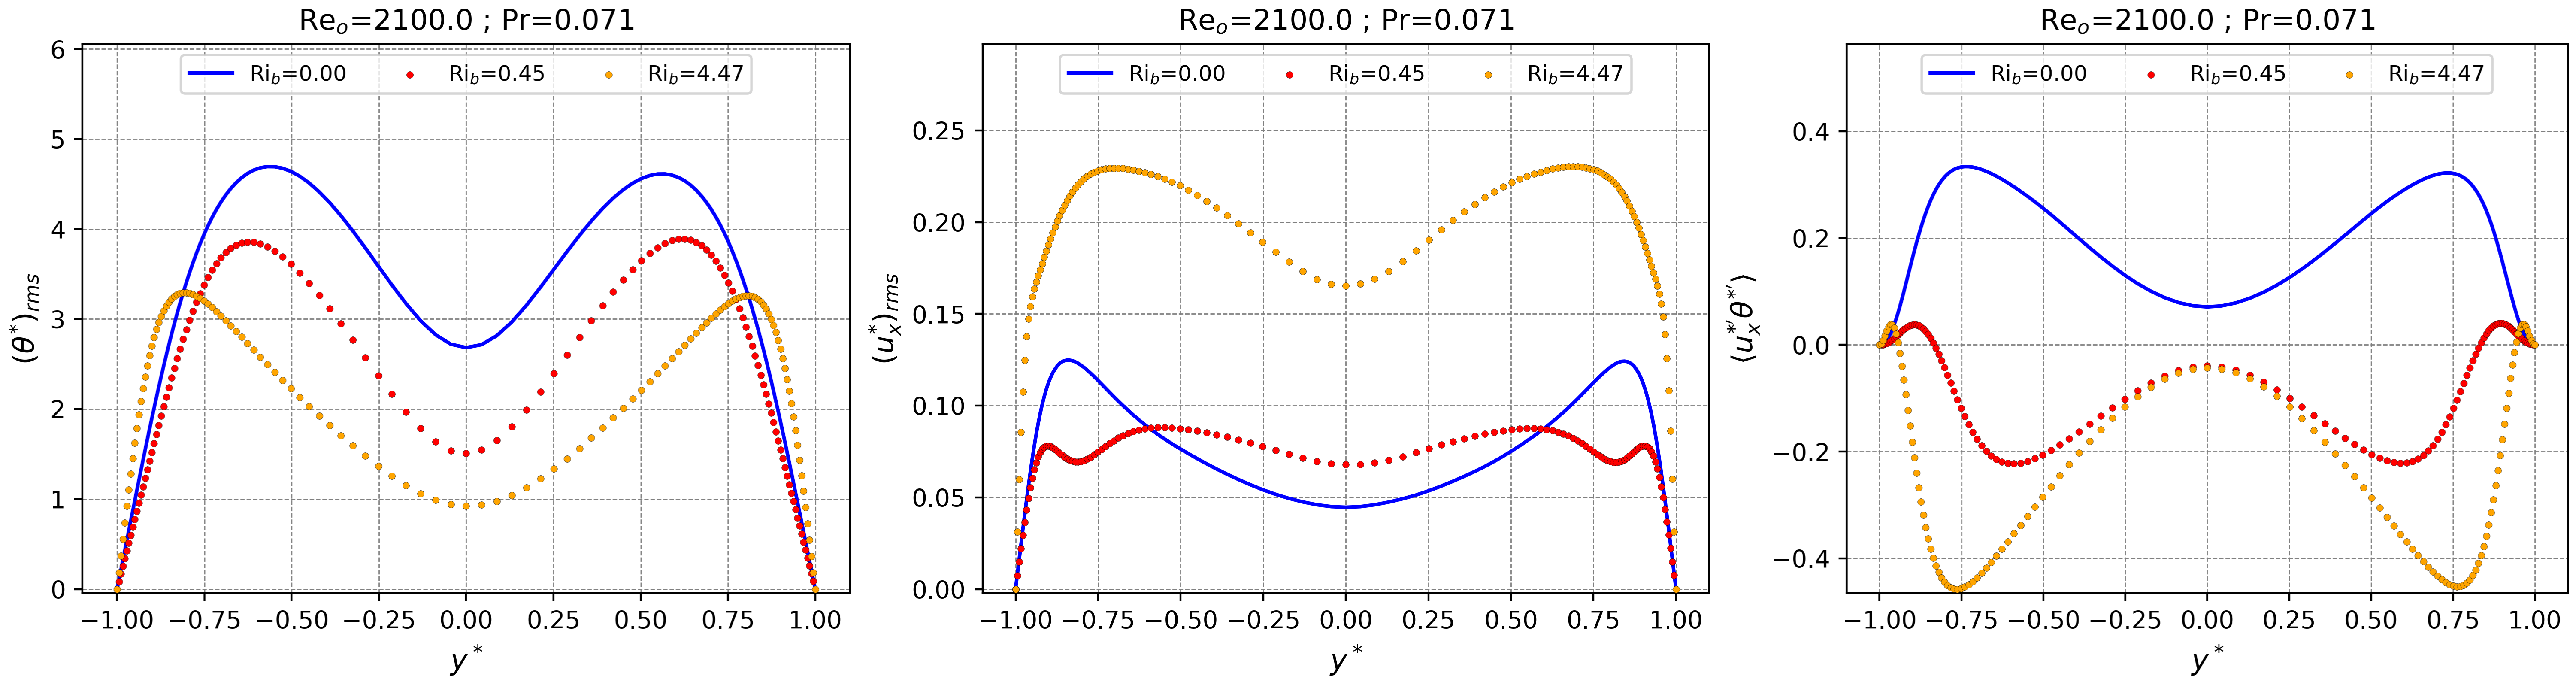
\includegraphics[width=\textwidth]{figures/apendices/developed/Re2100-Pr0071_merged_phif-uxf-uxphif.png}
  \caption{Perfiles de  $( \theta^*)_{\text{rms}}$,  $(u^*_x)_{\text{rms}}$ y   $\langle u^{* \prime}_x \theta^{* \prime} \rangle$.}
  \label{fig:profs-Re2100-Pr0071}
\end{figure}

%%%%%%%%%%%%%%%%%%%%%%%%%%%%%%%%%%%%%%%%%%

\subsection*{$\text{Re}=3150$ y $\text{Pr}=0\text{.}71$}

\begin{figure}[H]
  \centering
    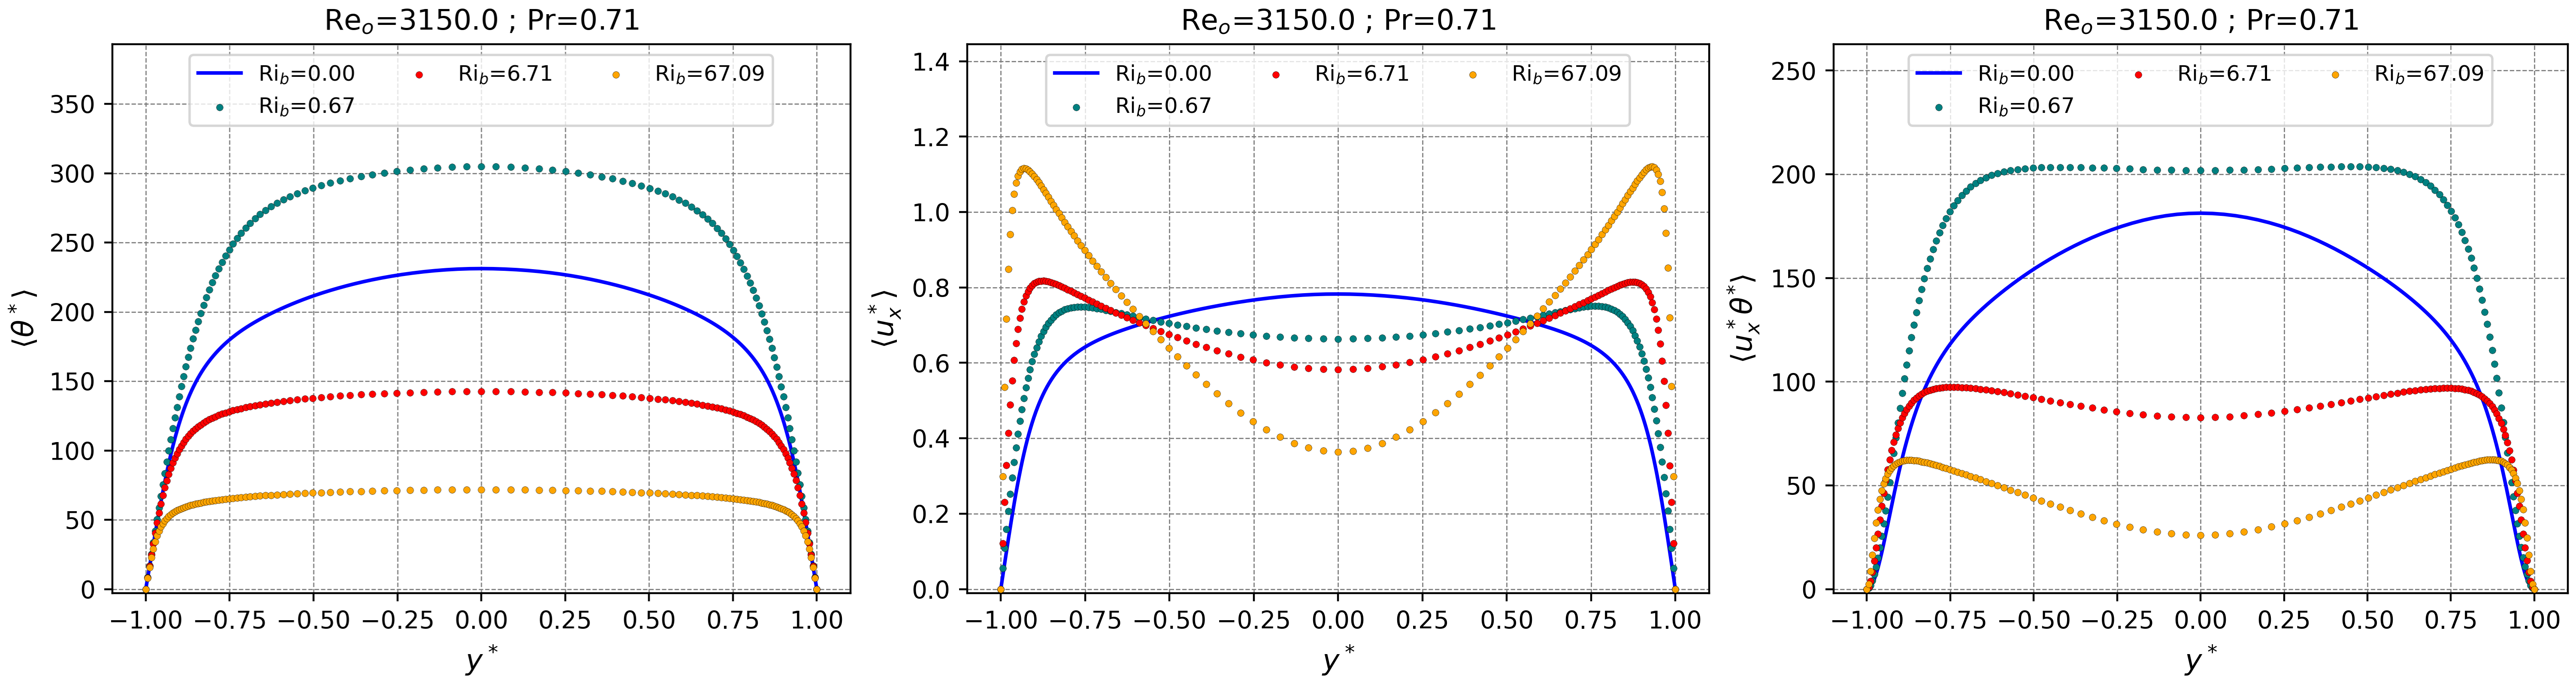
\includegraphics[width=\textwidth]{figures/apendices/developed/Re3150-Pr071_merged_phi-ux-uxphi.png}
  \caption{Perfiles de  $\langle \theta^* \rangle$,  $\langle u^*_x \rangle$ y   $\langle u^*_x \theta^* \rangle$.}
  \label{fig:profs-Re2100-Pr071}
\end{figure}

\begin{figure}[H]
  \centering
    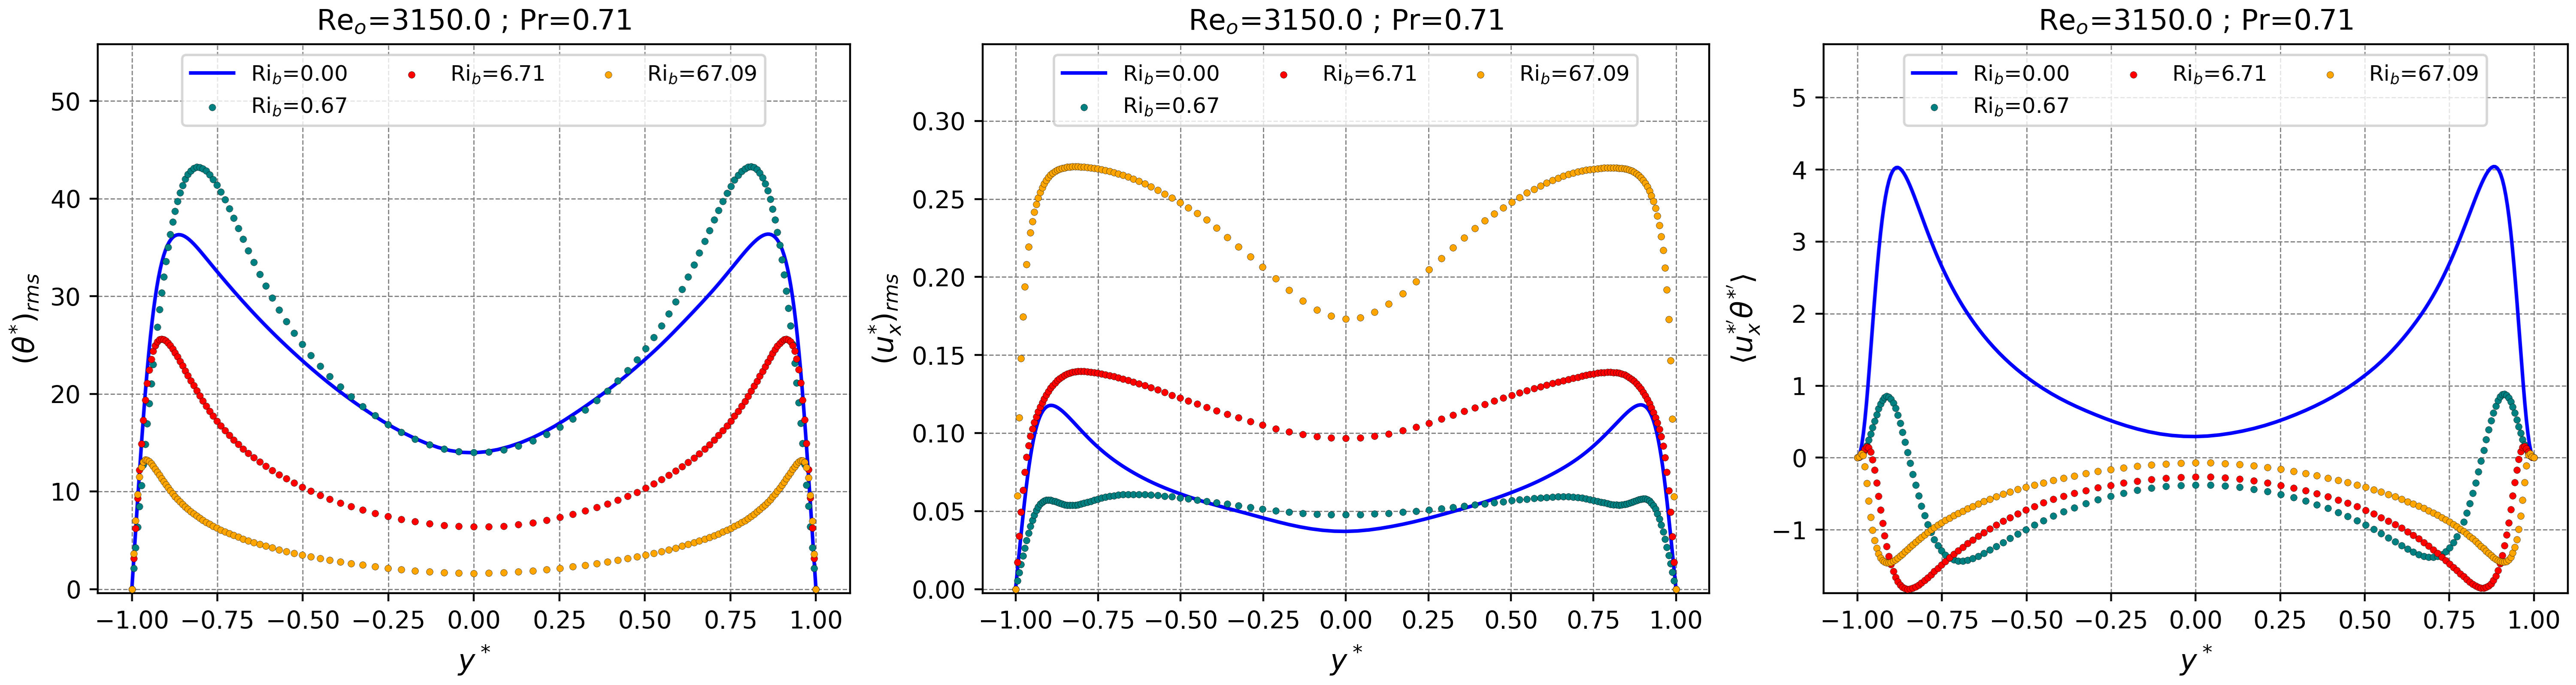
\includegraphics[width=\textwidth]{figures/apendices/developed/Re3150-Pr071_merged_phif-uxf-uxphif.png}
  \caption{Perfiles de  $( \theta^*)_{\text{rms}}$,  $(u^*_x)_{\text{rms}}$ y   $\langle u^{* \prime}_x \theta^{* \prime} \rangle$.}
  \label{fig:profs-Re2100-Pr071}
\end{figure}

\subsection*{$\text{Re}=3150$ y $\text{Pr}=0\text{.}071$}

\begin{figure}[H]
  \centering
    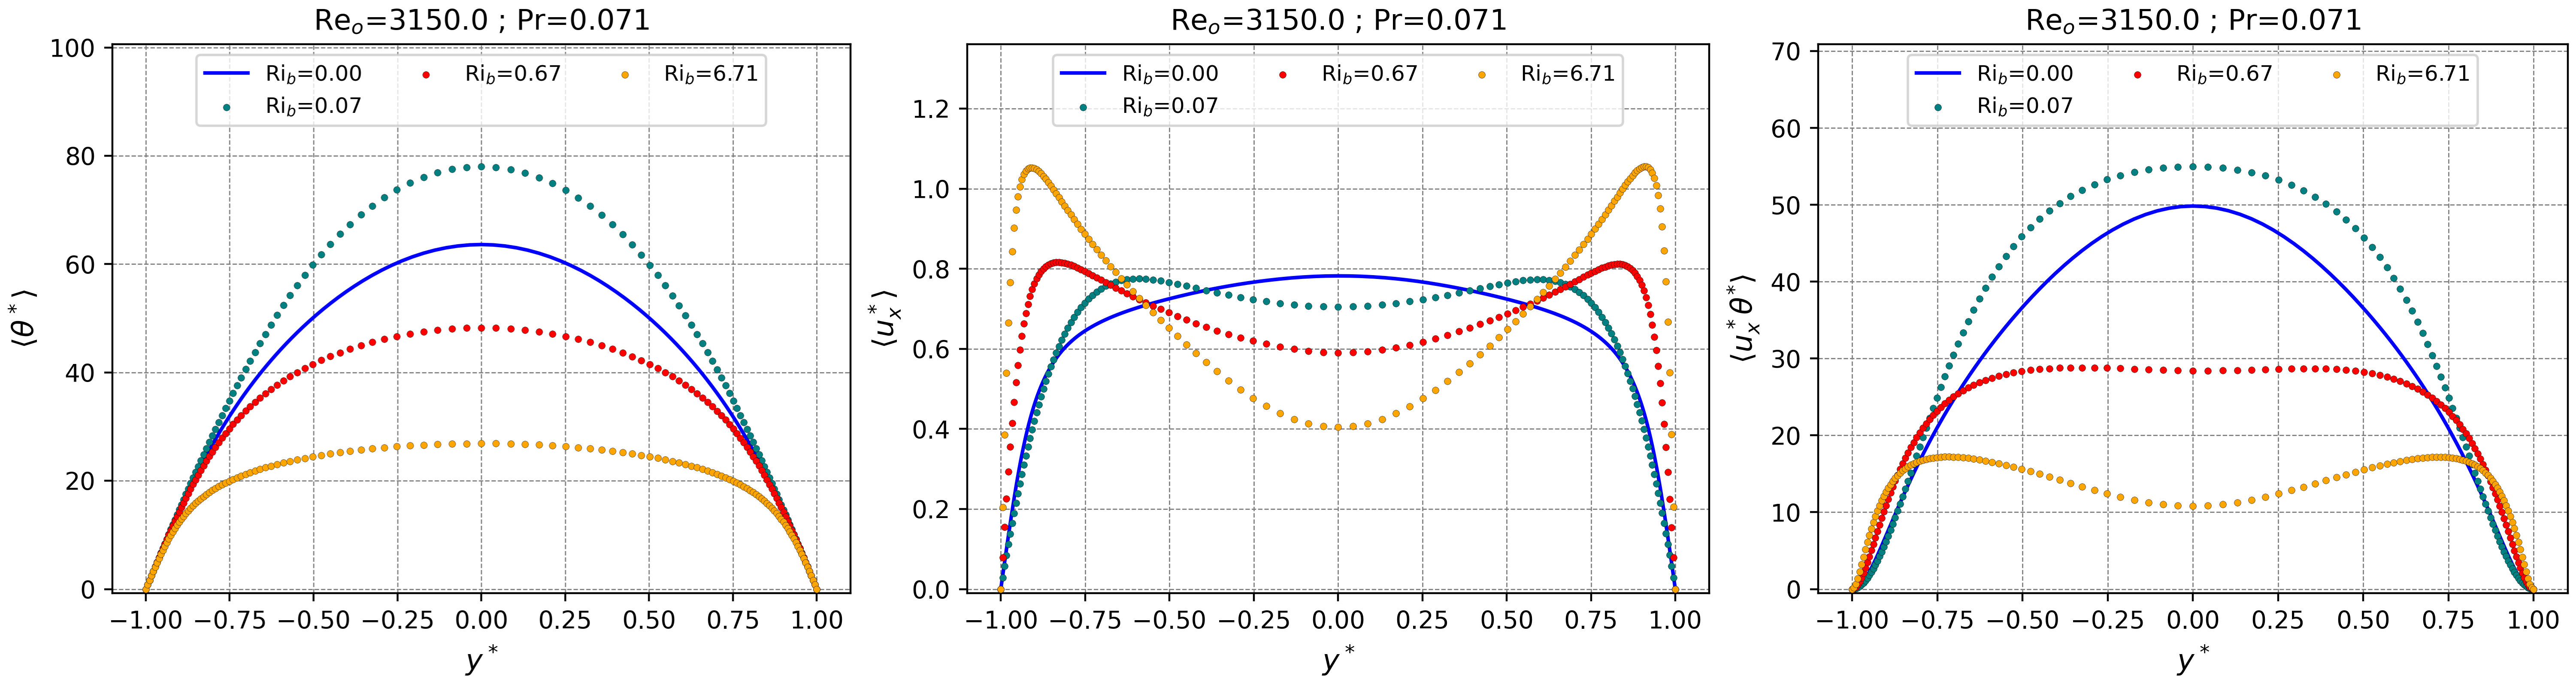
\includegraphics[width=\textwidth]{figures/apendices/developed/Re3150-Pr0071_merged_phi-ux-uxphi.png}
  \caption{Perfiles de  $\langle \theta^* \rangle$,  $\langle u^*_x \rangle$ y   $\langle u^*_x \theta^* \rangle$.}
  \label{fig:profs-Re3150-Pr0071}
\end{figure}

\begin{figure}[H]
  \centering
    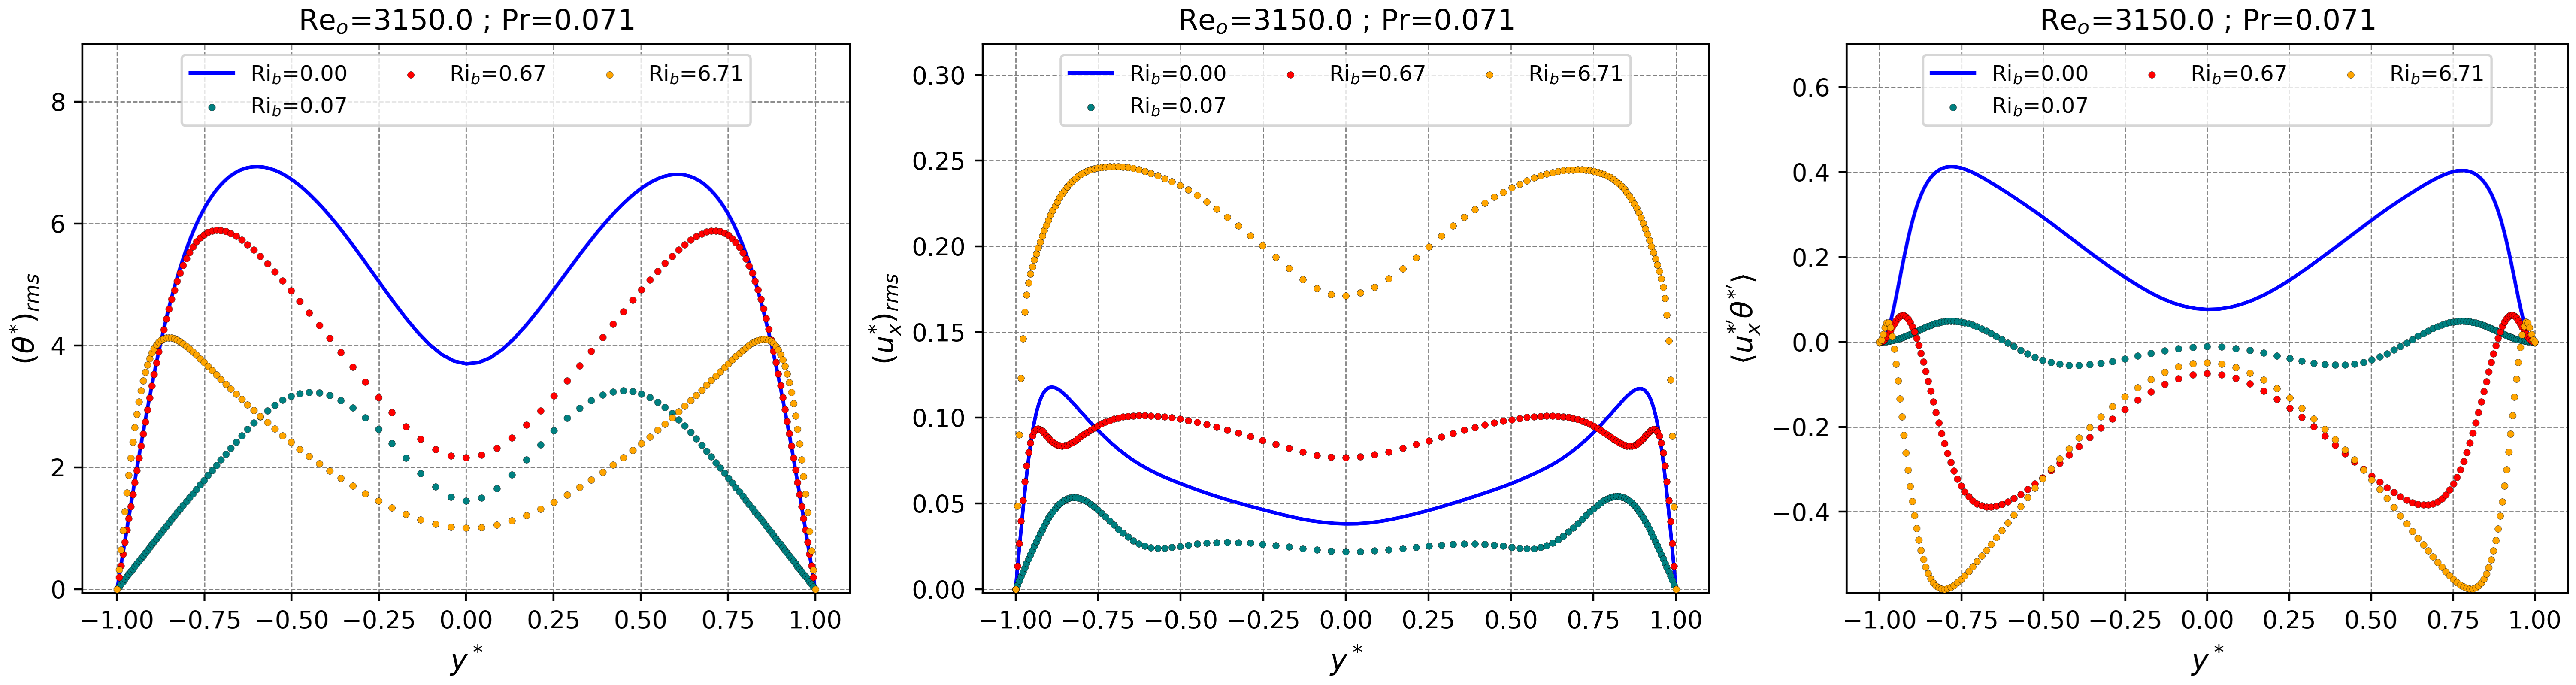
\includegraphics[width=\textwidth]{figures/apendices/developed/Re3150-Pr0071_merged_phif-uxf-uxphif.png}
  \caption{Perfiles de  $( \theta^*)_{\text{rms}}$,  $(u^*_x)_{\text{rms}}$ y  $\langle u^{* \prime}_x \theta^{* \prime} \rangle$.}
  \label{fig:profs-Re3150-Pr0071}
\end{figure}

%%%%%%%%%%%%%%%%%%%%%%%%%

\subsection*{$\text{Re}=4278$ y $\text{Pr}=0\text{.}71$}

\begin{figure}[H]
  \centering
    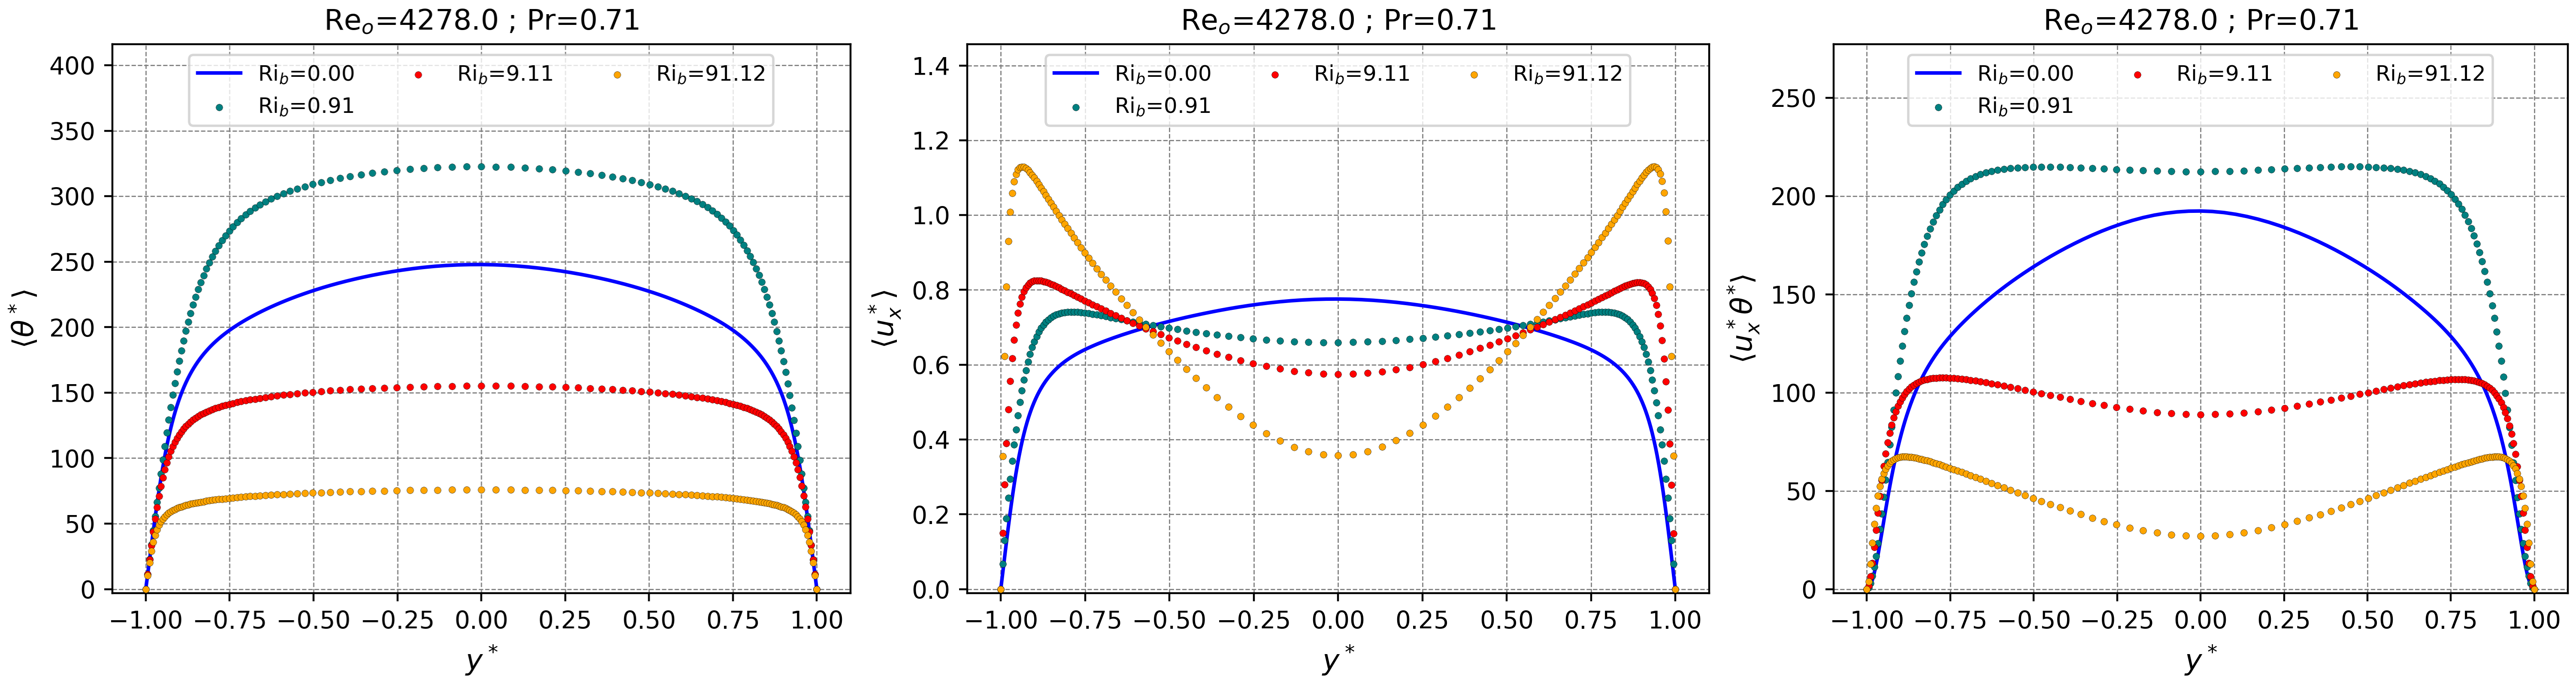
\includegraphics[width=\textwidth]{figures/apendices/developed/Re4278-Pr071_merged_phi-ux-uxphi.png}
  \caption{Perfiles de  $\langle \theta^* \rangle$,  $\langle u^*_x \rangle$ y   $\langle u^*_x \theta^* \rangle$.}
  \label{fig:profs-Re4278-Pr071}
\end{figure}

\begin{figure}[H]
  \centering
    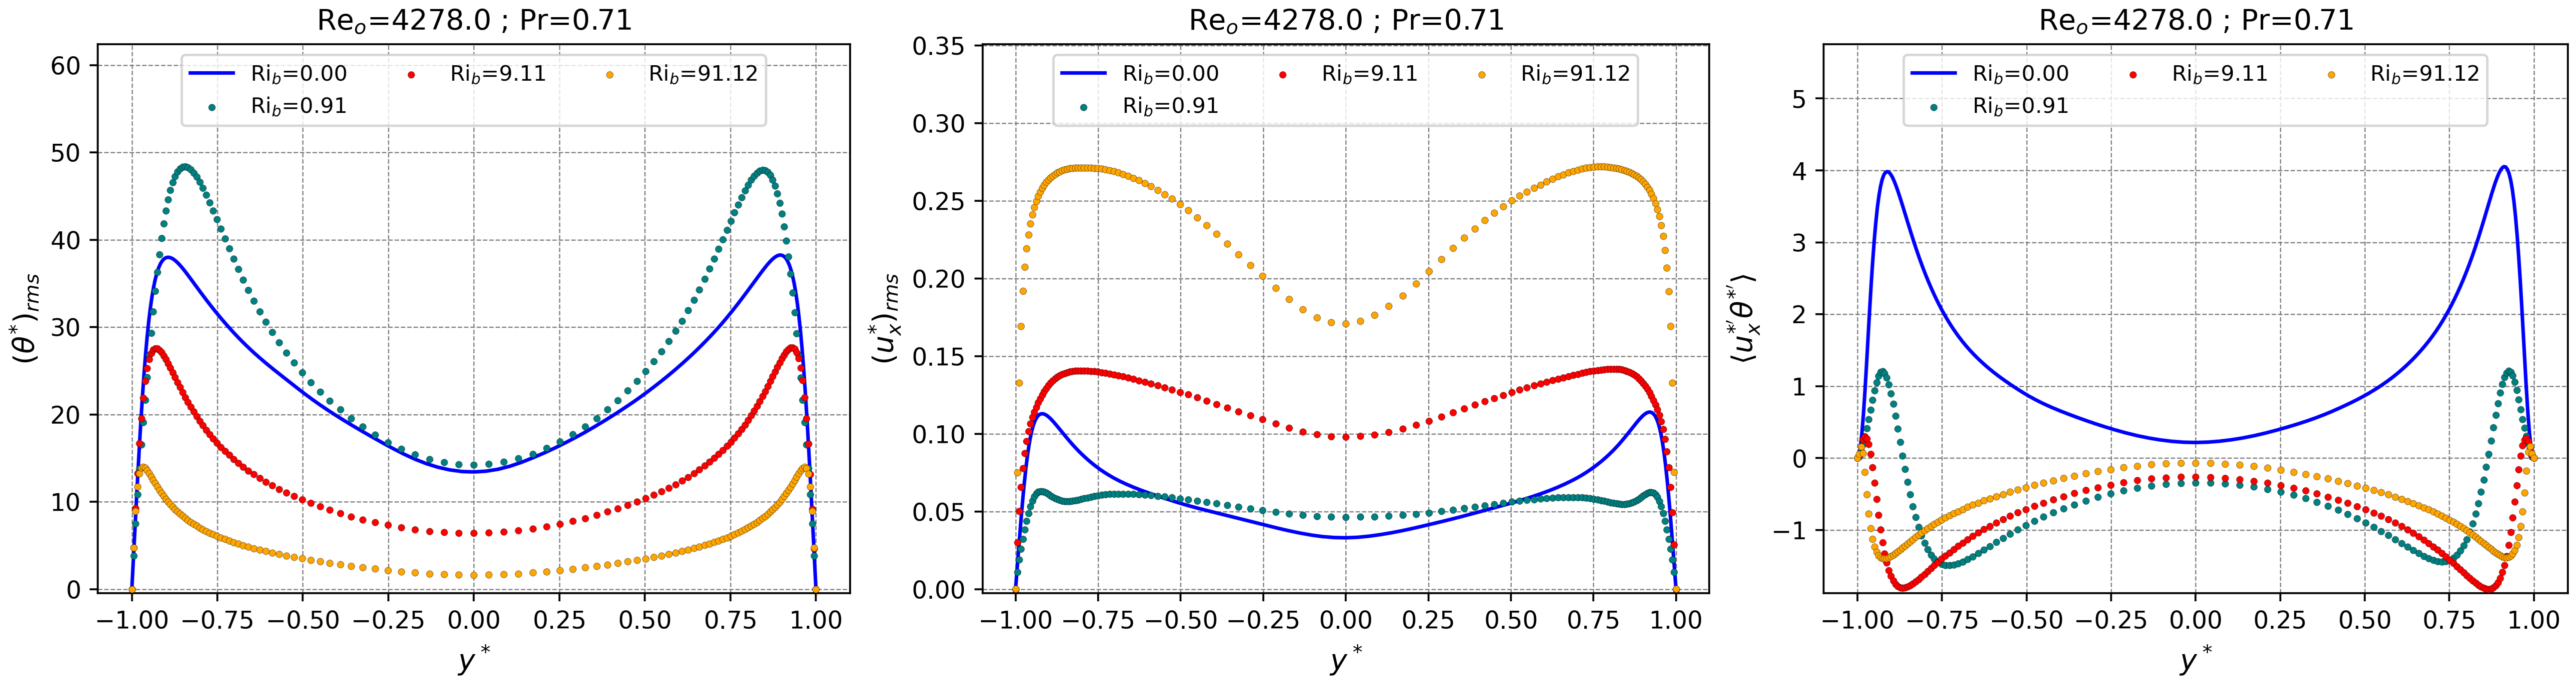
\includegraphics[width=\textwidth]{figures/apendices/developed/Re4278-Pr071_merged_phif-uxf-uxphif.png}
  \caption{Perfiles de  $( \theta^*)_{\text{rms}}$,  $(u^*_x)_{\text{rms}}$ y   $\langle u^{* \prime}_x \theta^{* \prime} \rangle$.}
  \label{fig:profs-Re4278-Pr071}
\end{figure}

\subsection*{$\text{Re}=4278$ y $\text{Pr}=0\text{.}071$}

\begin{figure}[H]
  \centering
    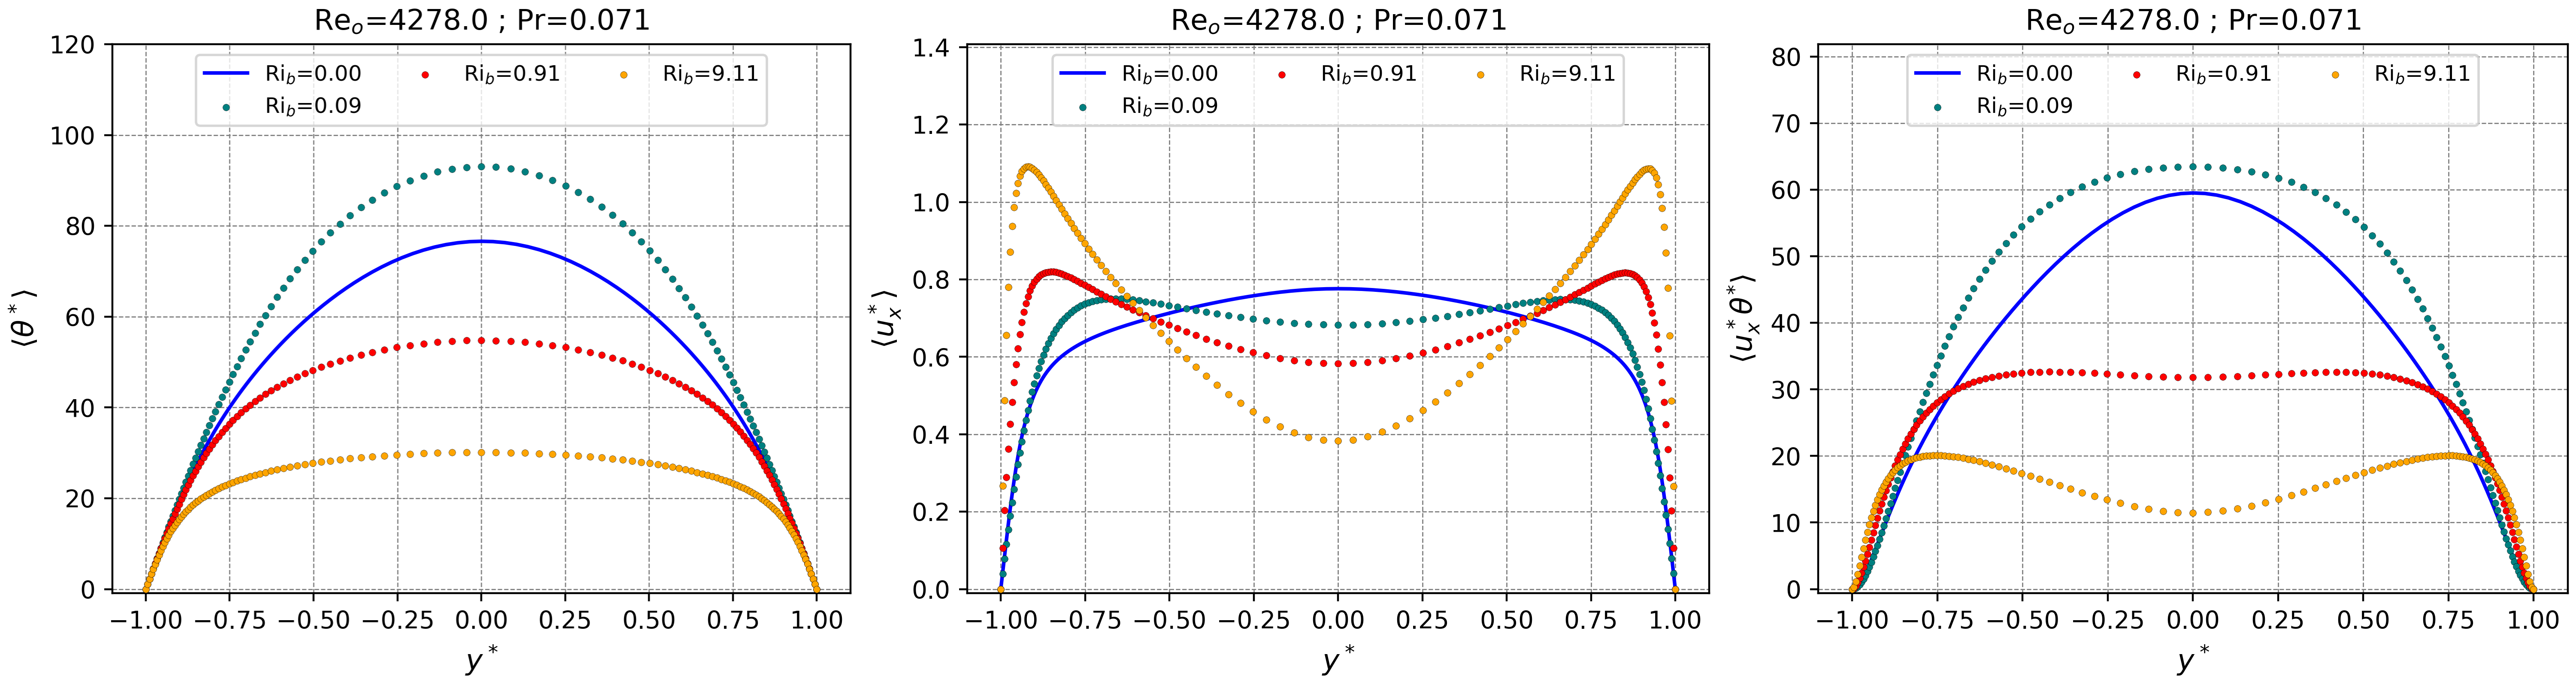
\includegraphics[width=\textwidth]{figures/apendices/developed/Re4278-Pr0071_merged_phi-ux-uxphi.png}
  \caption{Perfiles de  $\langle \theta^* \rangle$,  $\langle u^*_x \rangle$ y  $\langle u^*_x \theta^* \rangle$.}
  \label{fig:profs-Re4278-Pr0071}
\end{figure}

\begin{figure}[H]
  \centering
    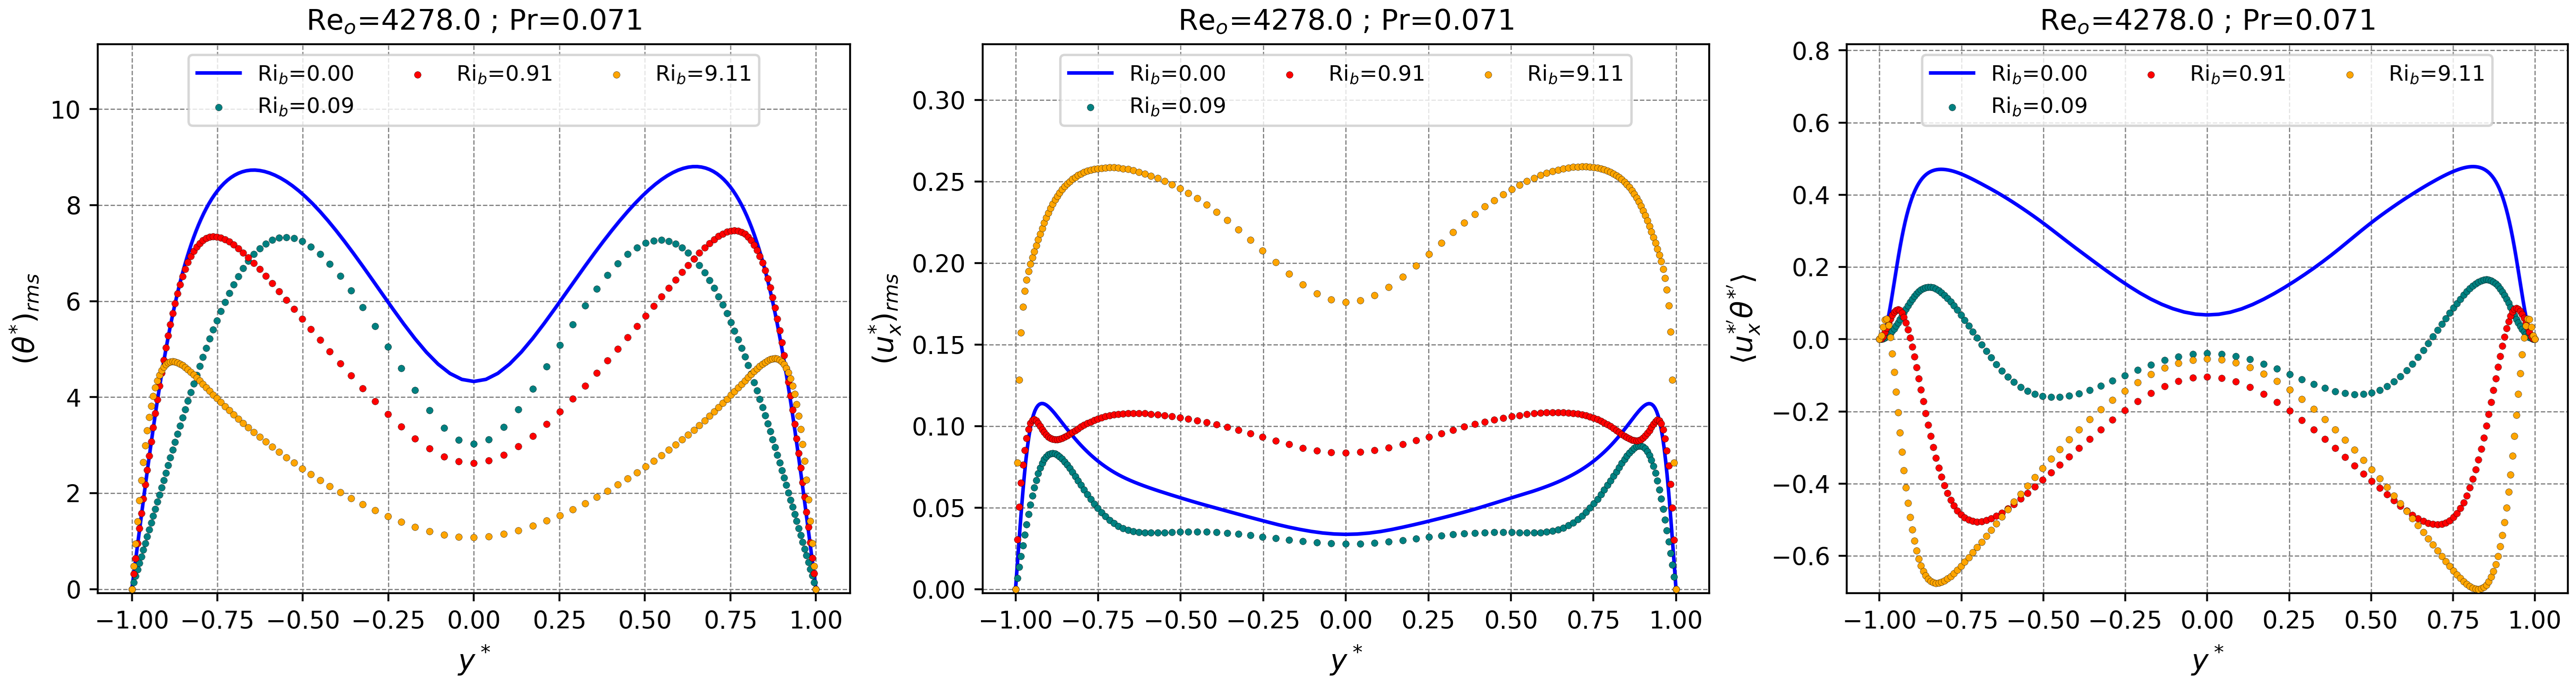
\includegraphics[width=\textwidth]{figures/apendices/developed/Re4278-Pr0071_merged_phif-uxf-uxphif.png}
  \caption{Perfiles de  $( \theta^*)_{\text{rms}}$,  $(u^*_x)_{\text{rms}}$ y  $\langle u^{* \prime}_x \theta^{* \prime} \rangle$.}
  \label{fig:profs-Re4278-Pr0071}
\end{figure}